\savestack{\figuretwo}{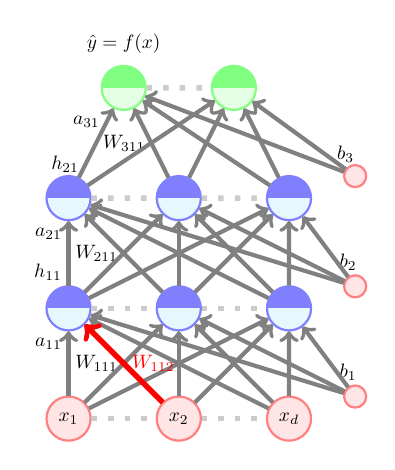
\begin{tikzpicture}[scale=0.7,transform shape]
	\tikzstyle{input_neuron}=[circle,draw=red!50,fill=red!10,thick,minimum size=8mm]
	\tikzstyle{hidden_neuron}=[circle,draw=blue!50,fill=cyan!10,thick,minimum size=8mm]
	\tikzstyle{output_neuron}=[circle,draw=green!50,fill=green!10,thick,minimum size=8mm]
	\tikzstyle{bias_neuron}=[circle,draw=red!50,fill=red!10,thick,minimum size=4mm]

	\tikzstyle{input}=[circle,draw=black!50,fill=black!20,thick,minimum size=8mm]

	\node [input_neuron] (neuron01) at (0,0) {$x_1$};
	\node [input_neuron] (neuron02) at (2,0){$x_2$};
	\node [input_neuron] (neuron03) at (4,0) {$x_d$};

	\node [bias_neuron] (neuron04) at (5.2,0.4) {};


	\node [hidden_neuron] (neuron11) at (0,2)  {};
	\node [hidden_neuron] (neuron12) at (2,2)  {};
	\node [hidden_neuron] (neuron13) at (4,2)  {};

	\node [bias_neuron] (neuron14) at (5.2,2.4) {};

	\begin{scope}
		\path[clip] (0,2) circle (4mm);
		\path[fill=blue!50] (-0.4,2) rectangle (0.4,2.4);
	\end{scope}
	\begin{scope}
		\path[clip] (2,2) circle (4mm);
		\path[fill=blue!50] (1.6,2) rectangle (2.4,2.4);
	\end{scope}
	\begin{scope}
		\path[clip] (4,2) circle (4mm);
		\path[fill=blue!50] (3.6,2) rectangle (4.4,2.4);
	\end{scope}


	\node [hidden_neuron] (neuron21) at (0,4)  {};
	\node [hidden_neuron] (neuron22) at (2,4)  {};
	\node [hidden_neuron] (neuron23) at (4,4)  {};

	\node [bias_neuron] (neuron24) at (5.2,4.4) {};


	\begin{scope}
		\path[clip] (0,4) circle (4mm);
		\path[fill=blue!50] (-0.4,4) rectangle (0.4,4.4);
	\end{scope}
	\begin{scope}
		\path[clip] (2,4) circle (4mm);
		\path[fill=blue!50] (1.6,4) rectangle (2.4,4.4);
	\end{scope}
	\begin{scope}
		\path[clip] (4,4) circle (4mm);
		\path[fill=blue!50] (3.6,4) rectangle (4.4,4.4);
	\end{scope}



	\node [output_neuron] (neuron31) at (1,6)  {};
	\node [output_neuron] (neuron32) at (3,6)  {};



	\begin{scope}
		\path[clip] (1,6) circle (4mm);
		\path[fill=green!50] (0.6,6) rectangle (1.4,6.4);
	\end{scope}
	\begin{scope}
		\path[clip] (3,6) circle (4mm);
		\path[fill=green!50] (2.6,6) rectangle (3.4,6.4);
	\end{scope}

	\draw[white,->] (neuron01) -- (neuron11) node[black,pos=.5,right]  {$W_{111}$} node[black,pos=0.8,left] {$a_{11}$};

	\draw[white,->] (neuron11) -- (neuron21) node[black,pos=.5,right] {$W_{211}$} node[black,pos=0.8,left] {$a_{21}$} node[black,pos=.2,left] {$h_{11}$};
	\draw[white,->] (neuron21) -- (neuron31) node[black,pos=.5,right] {$W_{311}$} node[black,pos=0.8,left] {$a_{31}$} node[black,pos=.2,left] {$h_{21}$};

	\draw[white,->] (neuron04) -- (neuron13) node[black,pos=0,right,above] {$b_1$};

	\draw[white,->] (neuron14) -- (neuron23) node[black,pos=0,right,above] {$b_2$};

	\draw[white,->] (neuron24) -- (neuron32) node[black,pos=0,right,above] {$b_3$};



	\draw[white,->] (neuron31) -- (1,6.5) node[black,pos=1,above] {$\hat{y} = f(x)$};
	%\draw[white,->] (neuron31) -- (3,6.5) node[black,pos=1,above] {$f(x)$};
	%node[pos=1.3,above,right] {$\mathscr{L}(\theta)$};

	\draw[black!20,line width=2pt,loosely dotted] (neuron01) -- (neuron02);
	\draw[black!20,line width=2pt,loosely dotted] (neuron02) -- (neuron03);
	\draw[black!20,line width=2pt,loosely dotted] (neuron11) -- (neuron12);
	\draw[black!20,line width=2pt,loosely dotted] (neuron12) -- (neuron13);
	\draw[black!20,line width=2pt,loosely dotted] (neuron21) -- (neuron22);
	\draw[black!20,line width=2pt,loosely dotted] (neuron22) -- (neuron23);
	\draw[black!20,line width=2pt,loosely dotted] (neuron31) -- (neuron32);


	\foreach \from in {neuron01,neuron02,neuron03,neuron04}
	\foreach \to in {neuron11,neuron12,neuron13}
	\draw [black!50,line width=1.5pt,->] (\from) -- (\to);

	\foreach \from in {neuron11,neuron12,neuron13,neuron14}
	\foreach \to in {neuron21,neuron22,neuron23}
	\draw [black!50,line width=1.5pt,->] (\from) -- (\to);

	\foreach \from in {neuron21,neuron22,neuron23,neuron24}
	\foreach \to in {neuron31,neuron32}
	\draw [black!50,line width=1.5pt,->] (\from) -- (\to);

	\draw [red,line width=2pt,->] (neuron02) -- (neuron11) node[pos=0.5,right] {$W_{112}$};

\end{tikzpicture}}
\savestack{\figurethree}{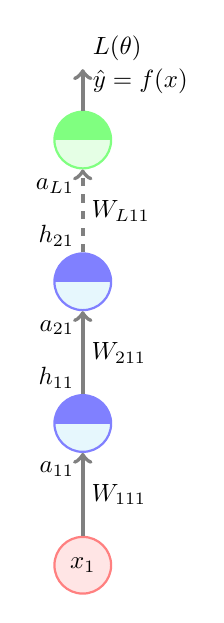
\begin{tikzpicture}[scale=0.9,transform shape]
	\tikzstyle{input_neuron}=[circle,draw=red!50,fill=red!10,thick,minimum size=8mm]
	\tikzstyle{hidden_neuron}=[circle,draw=blue!50,fill=cyan!10,thick,minimum size=8mm]
	\tikzstyle{output_neuron}=[circle,draw=green!50,fill=green!10,thick,minimum size=8mm]


	\node [input_neuron] (neuron01) at (0,0) {$x_1$};
	\node [hidden_neuron] (neuron11) at (0,2)  {};

	\begin{scope}
		\path[clip] (0,2) circle (4mm);
		\path[fill=blue!50] (-0.4,2) rectangle (0.4,2.4);
	\end{scope}


	\node [hidden_neuron] (neuron21) at (0,4)  {};


	\begin{scope}
		\path[clip] (0,4) circle (4mm);
		\path[fill=blue!50] (-0.4,4) rectangle (0.4,4.4);
	\end{scope}

	\node [output_neuron] (neuron31) at (0,6)  {};



	\begin{scope}
		\path[clip] (0,6) circle (4mm);
		\path[fill=green!50] (-0.4,6) rectangle (0.4,6.4);
	\end{scope}

	\draw[white,->] (neuron01) -- (neuron11) node[black,pos=.5,right]  {$W_{111}$} node[black,pos=0.8,left] {$a_{11}$};

	\draw[white,->] (neuron11) -- (neuron21) node[black,pos=.5,right] {$W_{211}$} node[black,pos=0.8,left] {$a_{21}$} node[black,pos=.2,left] {$h_{11}$};
	\draw[white,->] (neuron21) -- (neuron31) node[black,pos=.5,right] {$W_{L11}$} node[black,pos=0.8,left] {$a_{L1}$} node[black,pos=.2,left] {$h_{21}$};


	\draw[black!50,line width=1.5pt,->] (neuron31) -- (0,7) node[black,pos=0.7,right] {$\hat{y} = f(x)$} node[black,pos=1.5,above,right] {$\mathscr{L}(\theta)$};
	%\draw[white,->] (neuron31) -- (3,6.5) node[black,pos=1,above] {$f(x)$};
	%node[pos=1.3,above,right] {$\mathscr{L}(\theta)$};


	\foreach \from in {neuron01}
	\foreach \to in {neuron11}
	\draw [black!50,line width=1.5pt,->] (\from) -- (\to);

	\foreach \from in {neuron11}
	\foreach \to in {neuron21}
	\draw [black!50,line width=1.5pt,->] (\from) -- (\to);

	\foreach \from in {neuron21}
	\foreach \to in {neuron31}
	\draw [black!50,line width=1.5pt,dashed,->] (\from) -- (\to);


\end{tikzpicture}}

\begin{frame}
  \myheading{Module 4.4: Backpropagation (Intuition)}
\end{frame}

%Slide 19
\begin{frame}
  \begin{block}{We need to answer two questions}
    \begin{itemize}
      % \justifying
      \item How to choose the loss function $\mathscr{L}(\theta)$ ?
      \item \alert<2->{How to compute $\nabla \theta$ which is composed of $\nabla W_1, \nabla W_2, ..., \nabla W_{L-1} \in \mathbb{R}^{n \times n}, \nabla W_{L} \in \mathbb{R}^{n \times k},$ \\ $\nabla b_1, \nabla b_2, ..., \nabla b_{L-1} \in \mathbb{R}^n $ and $\nabla b_{L} \in \mathbb{R}^k$ ?}
    \end{itemize}
  \end{block}
\end{frame}

%Slide 20
\begin{frame}
  \begin{columns}
    \column{0.33\textwidth}
    \begin{overlayarea}{\textwidth}{\textheight}
      \begin{itemize}
        % \justifying
        \item<1-> Let us focus on this one weight.
        \item<2-> To learn this weight using SGD we need a formula for $\frac{\partial \mathscr{L}(\theta)}{ \partial W_{112}}$.
        \item<3-> We will see how to calculate this.
      \end{itemize}
    \end{overlayarea}

    \column{0.33\textwidth}

    \begin{overlayarea}{\textwidth}{\textheight}
      \makebox[\textwidth][c]{\usebox{\figuretwocontent}}
    \end{overlayarea}

    \column{0.33\textwidth}
    \begin{overlayarea}{\textwidth}{\textheight}
      \begin{algorithm}[H]
        \SetAlgoLined
        $t \leftarrow 0$\;
        $max\_iterations\leftarrow 1000$\;
        $Initialize \quad \theta_0$\;
        \color{black}
        \While{$t\texttt{++} < max\_iterations$}{
          $\theta_{t+1} \leftarrow \theta_{t} - \eta \nabla \theta_{t}$\;
        }
        \caption{gradient descent()}
      \end{algorithm}
    \end{overlayarea}
  \end{columns}
\end{frame}

%Slide 21
\begin{frame}
  \begin{columns}
    \column{0.53\textwidth}
    \begin{overlayarea}{\textwidth}{\textheight}
      \begin{itemize}[<+->]
      % \justifying
        \item First let us take the simple case when we have a deep but thin network.
        \item In this case it is easy to find the derivative by chain rule.
      \end{itemize}
      \begin{align*}
        \visible<3->{
        \frac{\partial \mathscr{L}(\theta)}{\partial W_{111}} & = \color<6>{red}{\color<4->{red}{\color<5>{red}{\frac{\partial \mathscr{L}(\theta)}{\partial \hat{y}} \frac{\partial \hat{y}}{\partial a_{L11}}} \color<6>{red}{\frac{\partial a_{L11}}{\partial h_{21}}} \color<5>{red}{\frac{\partial h_{21}}{\partial a_{21}} \frac{\partial a_{21}}{\partial h_{11}}} \color<4->{blue}{\frac{\partial h_{11}}{\partial a_{11}} \frac{\partial a_{11}}{\partial W_{111}}}}}
        }\\
        \visible<4->{
        \frac{\partial \mathscr{L}(\theta)}{\partial W_{111}} & = \color<4->{red}{\frac{\partial \mathscr{L}(\theta)}{\partial h_{11}}}
          \color<4->{blue}{\frac{\partial h_{11}}{\partial W_{111}}} ~~~~ \color<4->{black}\text{(just compressing the chain rule)}
        } \\
        \visible<5->{
        \frac{\partial \mathscr{L}(\theta)}{\partial W_{211}} & = \frac{\partial \mathscr{L}(\theta)}{\partial h_{21}}
          \frac{\partial h_{21}}{\partial W_{211}}
        } \\
        \visible<6->{
        \frac{\partial \mathscr{L}(\theta)}{\partial W_{L11}} & = \frac{\partial \mathscr{L}(\theta)}{\partial a_{L1}}
          \frac{\partial a_{L1}}{\partial W_{L11}}
        }
      \end{align*}
    \end{overlayarea}

    \column{0.47\textwidth}
    \begin{overlayarea}{\textwidth}{\textheight}
      % \only<1-6>{
          \makebox[\textwidth][c]{\usebox{\figurethreecontent}}
      % }
      % \only<7->{
      %   \begin{itemize}
      % \justifying
      %     \item <7->  Observe that if we come up with a generic formula:
      %         \begin{align*}
      %           \visible<7->{ & \frac{\partial \mathscr{L}(\theta)}{\partial h_{ij}} \text{\hspace{1em}(gradient w.r.t. hidden units)}}     \\
      %           \visible<8->{ & \frac{\partial \mathscr{L}(\theta)}{\partial a_{L,j}} \text{\hspace{0.1em} (gradient w.r.t. output units)}} \\
      %           \visible<9->{ & \frac{\partial h_{ij}}{\partial W_{ij}} \text{\hspace{1em} (gradient w.r.t. weights)}}
      %         \end{align*}
      %         \visible<10->{\noindent then we can compute all the required gradients}
      %     \item <11->  This is called the backpropagation algorithm because the loss gets propagated all the way back to the weights.
      %   \end{itemize}
      % }
    \end{overlayarea}
  \end{columns}
\end{frame}

%Slide 22
\begin{frame}
  Let us see an intuitive explanation of backpropagation before we get into the mathematical details
\end{frame}

%Slide 23
\begin{frame}
  \begin{columns}
    \column{0.6\textwidth}
    \begin{overlayarea}{\textwidth}{\textheight}
      \visible{
        \small{
          \begin{itemize}
            % \justifying

            % \justifying
            \item<1-> We get a certain loss at the output and we try to figure out who is responsible for this loss

            \item<2-> So, we talk to the output layer and say ``Hey! You are not producing the desired output, better take responsibility".

            \item<3-> The output layer says ``Well, I take responsibility for my part but please understand that I am only as the good as the hidden layer and weights below me". After all $\dots$
                $$ f(x) = \hat{y} = O(W_{L}h_{L-1}+b_{L}) $$

          \end{itemize}
        }
      }
    \end{overlayarea}

    \column{0.4\textwidth}
    \begin{overlayarea}{\textwidth}{\textheight}
      \hspace{-0.1in}
\tikzstyle{input_neuron}=[circle,draw=red!50,fill=red!10,thick,minimum size=5mm]
\tikzstyle{hidden_neuron}=[circle,draw=blue!50,fill=cyan!10,thick,minimum size=6mm]
\tikzstyle{output_neuron}=[circle,draw=green!50,fill=green!10,thick,minimum size=6mm]
\tikzstyle{bias_neuron}=[circle,draw=red!50,fill=red!10,thick,minimum size=2mm]
\tikzstyle{bias_hidden_neuron}=[circle,draw=blue!50,fill=cyan!10,thick,minimum size=2mm]
\tikzstyle{bias_hidden_neuron_hi}=[circle,draw=orange,fill=cyan!10,thick,minimum size=2mm]
\tikzstyle{input}=[circle,draw=black!50,fill=black!20,thick,minimum size=6mm]

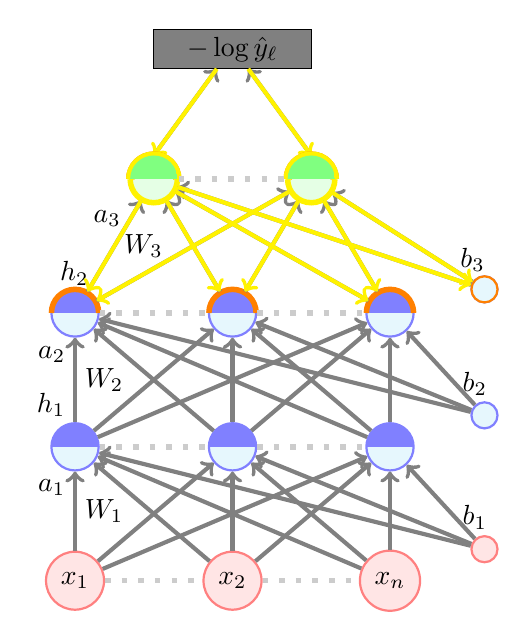
\begin{tikzpicture}
	\node [input_neuron] (neuron01) at (0,0) {$x_1$};
	\node [input_neuron] (neuron02) at (2,0){$x_2$};
	\node [input_neuron] (neuron03) at (4,0) {$x_n$};

	\node [bias_neuron] (neuron04) at (5.2,0.4) {};

	\node [hidden_neuron] (neuron11) at (0,1.7)  {};
	\node [hidden_neuron] (neuron12) at (2,1.7)  {};
	\node [hidden_neuron] (neuron13) at (4,1.7)  {};

	\node [bias_hidden_neuron] (neuron14) at (5.2,2.1) {};

	\begin{scope}
		\path[clip] (0,1.7) circle (3mm);
		\path[fill=blue!50] (-0.4,1.7) rectangle (0.3,2);
	\end{scope}
	\begin{scope}
		\path[clip] (2,1.7) circle (3mm);
		\path[fill=blue!50] (1.6,1.7) rectangle (2.3,2);
	\end{scope}
	\begin{scope}
		\path[clip] (4,1.7) circle (3mm);
		\path[fill=blue!50] (3.6,1.7) rectangle (4.3,2);
	\end{scope}


	\node [hidden_neuron] (neuron21) at (0,3.4)  {};
	\node [hidden_neuron] (neuron22) at (2,3.4)  {};
	\node [hidden_neuron] (neuron23) at (4,3.4)  {};

	\onslide<1-2>{\node [bias_hidden_neuron] (neuron24) at (5.2,3.7) {};}
	\onslide<3> {\node [bias_hidden_neuron_hi] (neuron24) at (5.2,3.7) {};}

	\begin{scope}
		\path[clip] (0,3.4) circle (3mm);
		\path[fill=blue!50] (-0.4,3.4) rectangle (0.4,3.7);
	\end{scope}
	\begin{scope}
		\path[clip] (2,3.4) circle (3mm);
		\path[fill=blue!50] (1.6,3.4) rectangle (2.4,3.7);
	\end{scope}
	\begin{scope}
		\path[clip] (4,3.4) circle (3mm);
		\path[fill=blue!50] (3.6,3.4) rectangle (4.4,3.7);
	\end{scope}


	\node [output_neuron] (neuron31) at (1,5.1)  {};
	\node [output_neuron] (neuron32) at (3,5.1)  {};
	\onslide<1->{\draw [fill=gray] (1, 7) rectangle (3, 6.5) node[pos=0.5] {$-\log\hat{y}_\ell$};}
	%\onslide<2->{\draw [fill=yellow!50] (1, 7) rectangle (3, 6.5) node[pos=0.5] {$-\log\hat{y}_\ell$};}
	\onslide<1>{\draw [black!50,line width=1.5pt,  ->] (1, 5.4) -- (1.8, 6.5);}
	\onslide<1>{\draw [black!50, line width=1.5pt, ->]  (3, 5.4) -- (2.2, 6.5);}
	\onslide<2->{\draw [yellow,line width=1.5pt,  ->] (1.8, 6.5) -- (1, 5.4);}
	\onslide<2->{\draw [yellow, line width=1.5pt, ->]  (2.2, 6.5) -- (3, 5.4);}
	\onslide<2>{\draw [orange, line width = 3] (1.3,5.1) arc (0:180:3mm) {};}
	\onslide<2>{\draw [orange, line width = 3] (3.3,5.1) arc (0:180:3mm) {};}
	\onslide<3>{\draw [yellow, line width = 3] (1.3,5.1) arc (0:180:3mm) {};}
	\onslide<3>{\draw [yellow, line width = 3] (3.3,5.1) arc (0:180:3mm) {};}
	\onslide<3>{\draw[yellow, line width = 2] (0.7, 5.1) arc (180:360:3mm){};}
	\onslide<3>{\draw[yellow, line width = 2] (2.7, 5.1) arc (180:360:3mm){};}
	\onslide<3>{\draw[orange, line width = 2] (0.3, 3.4) arc (0:180:3mm){};}
	\onslide<3>{\draw[orange, line width = 2] (2.3, 3.4) arc (0:180:3mm){};}
	\onslide<3>{\draw[orange, line width = 2] (4.3, 3.4) arc (0:180:3mm){};}


	\begin{scope}
		\path[clip] (1,5.1) circle (3mm);
		\path[fill=green!50] (0.6,5.1) rectangle (1.3,5.4);
	\end{scope}
	\begin{scope}
		\path[clip] (3,5.1) circle (3mm);
		\path[fill=green!50] (2.6,5.1) rectangle (3.3,5.4);
	\end{scope}

	\draw[white,->] (neuron01) -- (neuron11) node[black,pos=.5,right]  {$W_{1}$} node[black,pos=0.8,left] {$a_{1}$};

	\draw[white,->] (neuron11) -- (neuron21) node[black,pos=.5,right] {$W_{2}$} node[black,pos=0.8,left] {$a_{2}$} node[black,pos=.2,left] {$h_{1}$};
	\draw[white,->] (neuron21) -- (neuron31) node[black,pos=.5,right] {$W_{3}$} node[black,pos=0.8,left] {$a_{3}$} node[black,pos=.2,left] {$h_{2}$};

	\draw[white,->] (neuron04) -- (neuron13) node[black,pos=0,right,above] {$b_1$};

	\draw[white,->] (neuron14) -- (neuron23) node[black,pos=0,right,above] {$b_2$};

	\draw[white,->] (neuron24) -- (neuron32) node[black,pos=0,right,above] {$b_3$};

	\draw[black!20,line width=2pt,loosely dotted] (neuron01) -- (neuron02);
	\draw[black!20,line width=2pt,loosely dotted] (neuron02) -- (neuron03);
	\draw[black!20,line width=2pt,loosely dotted] (neuron11) -- (neuron12);
	\draw[black!20,line width=2pt,loosely dotted] (neuron12) -- (neuron13);
	\draw[black!20,line width=2pt,loosely dotted] (neuron21) -- (neuron22);
	\draw[black!20,line width=2pt,loosely dotted] (neuron22) -- (neuron23);
	\draw[black!20,line width=2pt,loosely dotted] (neuron31) -- (neuron32);


	\foreach \from in {neuron01,neuron02,neuron03,neuron04}
	\foreach \to in {neuron11,neuron12,neuron13}
	\draw [black!50,line width=1.5pt,->] (\from) -- (\to);

	\foreach \from in {neuron11,neuron12,neuron13,neuron14}
	\foreach \to in {neuron21,neuron22,neuron23}
	\draw [black!50,line width=1.5pt,->] (\from) -- (\to);

	\foreach \from in {neuron21,neuron24,neuron23, neuron22}
	\foreach \to in {neuron31,neuron32}
		{\onslide<1-2>{\draw [black!50,line width=1.5pt,->] (\from) -- (\to);}}

	\foreach \from in {neuron21,neuron24,neuron23, neuron22}
	\foreach \to in {neuron31,neuron32}
		{\onslide<3>{\draw [yellow,line width=1.5pt,->] (\to) -- (\from);}}


\end{tikzpicture}

    \end{overlayarea}
  \end{columns}
\end{frame}


%Slide 24
\begin{frame}
  \begin{columns}
    \column{0.6\textwidth}
    \begin{overlayarea}{\textwidth}{\textheight}
      \footnotesize{
        \begin{itemize}
          % \justifying
          \item So, we talk to $W_{L},b_{L}$ and $h_{L}$ and ask them ``What is wrong with you?"
          \item<2-> $W_{L}$ and $b_{L}$ take full responsibility but $h_{L}$ says ``Well, please understand that I am only as good as the pre-activation layer"
          \item<3-> The pre-activation layer in turn says that I am only as good as the hidden layer and weights below me.
          \item<4-> We continue in this manner and realize that the responsibility lies with all the weights and biases (i.e. all the parameters of the model)
          \item<5-> But instead of talking to them directly, it is easier to talk to them through the hidden layers and output layers (and this is exactly what the chain rule allows us to do)
              \visible<6->{
                \begin{align*}
                  \underbrace{\frac{\partial \mathscr{L}(\theta)}{\partial W_{11}}}_
                  {\substack{\text{Talk to the}\\ \text{weight directly}}}
                  =
                  \underbrace{\frac{\partial \mathscr{L}(\theta)}{\partial f(x)} \frac{\partial f(x)}{\partial a_{3}}}_
                  {\substack{\text{Talk to the} \\ \text{output layer}}}
                  \underbrace{\frac{\partial a_{3}}{\partial h_{2}} \frac{\partial h_{2}}{\partial a_{2}}}_
                  {\substack{\text{Talk to the} \\ \text{previous hidden} \\ \text{layer}}}
                  \underbrace{\frac{\partial a_{2}}{\partial h_{1}} \frac{\partial h_{1}}{\partial a_{1}}}_
                  {\substack{\text{Talk to the} \\ \text{previous} \\ \text{hidden layer}}}
                  \underbrace{\frac{\partial a_{1}}{\partial W_{11}}}_
                  {\substack{\text{and now} \\ \text{talk to} \\ \text{the} \\ \text{weights}}}
                \end{align*}
              }
        \end{itemize}
      }
    \end{overlayarea}

    \column{0.4\textwidth}
    \begin{overlayarea}{\textwidth}{\textheight}
      \hspace{-0.1in}
\tikzstyle{input_neuron}=[circle,draw=red!50,fill=red!10,thick,minimum size=5mm]
\tikzstyle{hidden_neuron}=[circle,draw=blue!50,fill=cyan!10,thick,minimum size=6mm]
\tikzstyle{output_neuron}=[circle,draw=green!50,fill=green!10,thick,minimum size=6mm]
\tikzstyle{bias_neuron}=[circle,draw=red!50,fill=red!10,thick,minimum size=2mm]
\tikzstyle{bias_hidden_neuron}=[circle,draw=blue!50,fill=cyan!10,thick,minimum size=2mm]
\tikzstyle{bias_hidden_neuron_hi}=[circle,draw=orange,fill=cyan!10,thick,minimum size=2mm]
\tikzstyle{bias_hidden_neuron_hi_old}=[circle,draw=yellow,fill=cyan!10,thick,minimum size=2mm]
\tikzstyle{input}=[circle,draw=black!50,fill=black!20,thick,minimum size=6mm]
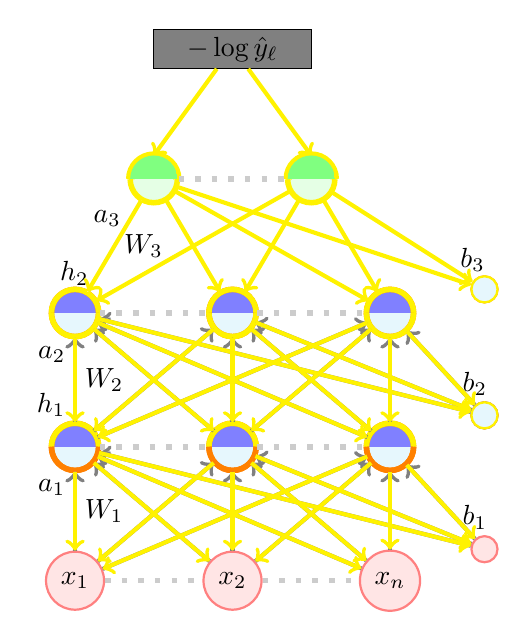
\begin{tikzpicture}
	\node [input_neuron] (neuron01) at (0,0) {$x_1$};
	\node [input_neuron] (neuron02) at (2,0){$x_2$};
	\node [input_neuron] (neuron03) at (4,0) {$x_n$};

	\node [bias_neuron] (neuron04) at (5.2,0.4) {};

	\node [hidden_neuron] (neuron11) at (0,1.7)  {};
	\node [hidden_neuron] (neuron12) at (2,1.7)  {};
	\node [hidden_neuron] (neuron13) at (4,1.7)  {};

	\node [bias_hidden_neuron] (neuron14) at (5.2,2.1) {};

	\begin{scope}
		\path[clip] (0,1.7) circle (3mm);
		\path[fill=blue!50] (-0.4,1.7) rectangle (0.3,2);
	\end{scope}
	\begin{scope}
		\path[clip] (2,1.7) circle (3mm);
		\path[fill=blue!50] (1.6,1.7) rectangle (2.3,2);
	\end{scope}
	\begin{scope}
		\path[clip] (4,1.7) circle (3mm);
		\path[fill=blue!50] (3.6,1.7) rectangle (4.3,2);
	\end{scope}


	\node [hidden_neuron] (neuron21) at (0,3.4)  {};
	\node [hidden_neuron] (neuron22) at (2,3.4)  {};
	\node [hidden_neuron] (neuron23) at (4,3.4)  {};


	\onslide<1> {\node [bias_hidden_neuron_hi] (neuron24) at (5.2,3.7) {};}
	\onslide<2-> {\node [bias_hidden_neuron_hi_old] (neuron24) at (5.2,3.7) {};}
	\begin{scope}
		\path[clip] (0,3.4) circle (3mm);
		\path[fill=blue!50] (-0.4,3.4) rectangle (0.4,3.7);
	\end{scope}
	\begin{scope}
		\path[clip] (2,3.4) circle (3mm);
		\path[fill=blue!50] (1.6,3.4) rectangle (2.4,3.7);
	\end{scope}
	\begin{scope}
		\path[clip] (4,3.4) circle (3mm);
		\path[fill=blue!50] (3.6,3.4) rectangle (4.4,3.7);
	\end{scope}


	\node [output_neuron] (neuron31) at (1,5.1)  {};
	\node [output_neuron] (neuron32) at (3,5.1)  {};
	\onslide<1->{\draw [fill=gray] (1, 7) rectangle (3, 6.5) node[pos=0.5] {$-\log\hat{y}_\ell$};}

	\onslide<1->{\draw [yellow,line width=1.5pt,  ->] (1.8, 6.5) -- (1, 5.4);}
	\onslide<1->{\draw [yellow, line width=1.5pt, ->]  (2.2, 6.5) -- (3, 5.4);}

	\onslide<1->{\draw [yellow, line width = 3] (1.3,5.1) arc (0:180:3mm) {};}
	\onslide<1->{\draw [yellow, line width = 3] (3.3,5.1) arc (0:180:3mm) {};}
	\onslide<1->{\draw[yellow, line width = 2] (0.7, 5.1) arc (180:360:3mm){};}
	\onslide<1->{\draw[yellow, line width = 2] (2.7, 5.1) arc (180:360:3mm){};}
	\onslide<1->{\draw[orange, line width = 2] (0.3, 3.4) arc (0:180:3mm){};}
	\onslide<1->{\draw[orange, line width = 2] (2.3, 3.4) arc (0:180:3mm){};}
	\onslide<1->{\draw[orange, line width = 2] (4.3, 3.4) arc (0:180:3mm){};}

	\onslide<2->{\draw[yellow, line width = 2] (0.3, 3.4) arc (0:180:3mm){};}
	\onslide<2->{\draw[yellow, line width = 2] (2.3, 3.4) arc (0:180:3mm){};}
	\onslide<2->{\draw[yellow, line width = 2] (4.3, 3.4) arc (0:180:3mm){};}
	\onslide<2>{\draw[orange, line width = 2] (-0.3, 3.4) arc (180:360:3mm){};}
	\onslide<2>{\draw[orange, line width = 2] (1.7, 3.4) arc (180:360:3mm){};}
	\onslide<2>{\draw[orange, line width = 2] (3.7, 3.4) arc (180:360:3mm){};}
	\onslide<3->{\draw[yellow, line width = 2] (-0.3, 3.4) arc (180:360:3mm){};}
	\onslide<3->{\draw[yellow, line width = 2] (1.7, 3.4) arc (180:360:3mm){};}
	\onslide<3->{\draw[yellow, line width = 2] (3.7, 3.4) arc (180:360:3mm){};}

	\onslide<3>{\draw[orange, line width = 2] (0.3, 1.7) arc (0:180:3mm){};}
	\onslide<3>{\draw[orange, line width = 2] (2.3, 1.7) arc (0:180:3mm){};}
	\onslide<3>{\draw[orange, line width = 2] (4.3, 1.7) arc (0:180:3mm){};}
	\onslide<3> {\node [bias_hidden_neuron_hi] (neuron14) at (5.2,2.1) {};}

	\onslide<4->{\draw[yellow, line width = 2] (0.3, 1.7) arc (0:180:3mm){};}
	\onslide<4->{\draw[yellow, line width = 2] (2.3, 1.7) arc (0:180:3mm){};}
	\onslide<4->{\draw[yellow, line width = 2] (4.3, 1.7) arc (0:180:3mm){};}
	\onslide<4-> {\node [bias_hidden_neuron_hi_old] (neuron14) at (5.2,2.1) {};}

	\onslide<4>{\draw[orange, line width = 2] (-0.3, 1.7) arc (180:360:3mm){};}
	\onslide<4>{\draw[orange, line width = 2] (1.7, 1.7) arc (180:360:3mm){};}
	\onslide<4>{\draw[orange, line width = 2] (3.7, 1.7) arc (180:360:3mm){};}

	\onslide<5->{\draw[orange, line width = 2] (-0.3, 1.7) arc (180:360:3mm){};}
	\onslide<5->{\draw[orange, line width = 2] (1.7, 1.7) arc (180:360:3mm){};}
	\onslide<5->{\draw[orange, line width = 2] (3.7, 1.7) arc (180:360:3mm){};}

	\begin{scope}
		\path[clip] (1,5.1) circle (3mm);
		\path[fill=green!50] (0.6,5.1) rectangle (1.3,5.4);
	\end{scope}
	\begin{scope}
		\path[clip] (3,5.1) circle (3mm);
		\path[fill=green!50] (2.6,5.1) rectangle (3.3,5.4);
	\end{scope}

	\draw[white,->] (neuron01) -- (neuron11) node[black,pos=.5,right]  {$W_{1}$} node[black,pos=0.8,left] {$a_{1}$};

	\draw[white,->] (neuron11) -- (neuron21) node[black,pos=.5,right] {$W_{2}$} node[black,pos=0.8,left] {$a_{2}$} node[black,pos=.2,left] {$h_{1}$};
	\draw[white,->] (neuron21) -- (neuron31) node[black,pos=.5,right] {$W_{3}$} node[black,pos=0.8,left] {$a_{3}$} node[black,pos=.2,left] {$h_{2}$};

	\draw[white,->] (neuron04) -- (neuron13) node[black,pos=0,right,above] {$b_1$};

	\draw[white,->] (neuron14) -- (neuron23) node[black,pos=0,right,above] {$b_2$};

	\draw[white,->] (neuron24) -- (neuron32) node[black,pos=0,right,above] {$b_3$};


	%\draw[white,->] (neuron31) -- (2.4.9) node[black,pos=1,above] {y };
	%\draw[white,->] (neuron31) -- (3,6.5) node[black,pos=1,above] {$f(x)$};
	%node[pos=1.3,above,right] {$\mathscr{L}(\theta)$};

	\draw[black!20,line width=2pt,loosely dotted] (neuron01) -- (neuron02);
	\draw[black!20,line width=2pt,loosely dotted] (neuron02) -- (neuron03);
	\draw[black!20,line width=2pt,loosely dotted] (neuron11) -- (neuron12);
	\draw[black!20,line width=2pt,loosely dotted] (neuron12) -- (neuron13);
	\draw[black!20,line width=2pt,loosely dotted] (neuron21) -- (neuron22);
	\draw[black!20,line width=2pt,loosely dotted] (neuron22) -- (neuron23);
	\draw[black!20,line width=2pt,loosely dotted] (neuron31) -- (neuron32);


	\foreach \from in {neuron01,neuron02,neuron03,neuron04}
	\foreach \to in {neuron11,neuron12,neuron13}
		{\onslide<1-4>{\draw [black!50,line width=1.5pt,->] (\from) -- (\to);}}


	\foreach \from in {neuron01,neuron02,neuron03,neuron04}
	\foreach \to in {neuron11,neuron12,neuron13}
		{\onslide<5->{\draw [yellow,line width=1.5pt,->] (\to) -- (\from);}}

	\foreach \from in {neuron11,neuron12,neuron13,neuron14}
	\foreach \to in {neuron21,neuron22,neuron23}
		{\onslide<1-2>{\draw [black!50,line width=1.5pt,->] (\from) -- (\to);}}

	\foreach \from in {neuron11,neuron12,neuron13,neuron14}
	\foreach \to in {neuron21,neuron22,neuron23}
		{\onslide<3->{\draw [yellow, line width=1.5pt,->] (\to) -- (\from);}}


	%\foreach \from in {neuron21,neuron24,neuron23, neuron22}
	%	\foreach \to in {neuron31,neuron32}
	%		{\onslide<1-2>{\draw [black!50,line width=1.5pt,->] (\from) -- (\to);}}

	\foreach \from in {neuron21,neuron24,neuron23, neuron22}
	\foreach \to in {neuron31,neuron32}
		{\onslide<1->{\draw [yellow,line width=1.5pt,->] (\to) -- (\from);}}


\end{tikzpicture}

    \end{overlayarea}
  \end{columns}
\end{frame}

%Slide 25
\begin{frame}
  \begin{overlayarea}{\textwidth}{\textheight}
    \visible<2->{\textbf{Quantities of interest (roadmap for the remaining part):}}
    \begin{itemize}
      % \justifying
      \item<3-> Gradient w.r.t. output units
      \item<4-> Gradient w.r.t. hidden units
      \item<5-> Gradient w.r.t. weights and biases
    \end{itemize}

    \begin{align*}
      \underbrace{\frac{\partial \mathscr{L}(\theta)}{\partial W_{11}}}_
      {\substack{\text{Talk to the}\\ \text{weight directly}}}
      =
      \underbrace{\frac{\partial \mathscr{L}(\theta)}{\partial \hat{y}} \frac{\partial \hat{y}}{\partial a_{3}}}_
        {\substack{\text{Talk to the} \\ \text{output layer}}}
      \underbrace{\frac{\partial a_{3}}{\partial h_{2}} \frac{\partial h_{2}}{\partial a_{2}}}_
      {\substack{\text{Talk to the} \\ \text{previous hidden} \\ \text{layer}}}
      \underbrace{\frac{\partial a_{2}}{\partial h_{1}} \frac{\partial h_{1}}{\partial a_{1}}}_
      {\substack{\text{Talk to the} \\ \text{previous} \\ \text{hidden layer}}}
      \underbrace{\frac{\partial a_{1}}{\partial W_{11}}}_
      {\substack{\text{and now} \\ \text{talk to} \\ \text{the} \\ \text{weights}}}
    \end{align*}
    
    \begin{itemize}
      % \justifying
      \item<6-> Our focus is on \textit{Cross entropy loss} and \textit{Softmax} output.
    \end{itemize}

  \end{overlayarea}
\end{frame}